 
\section{Conceptkeuze en ontwerp}
De lijst met productvereisten hielp bij het vinden van het beste idee. Het ontwerp dat het best voldeed aan de vereisten, een vierwieler met een stuurmechanisme gelijkaardig aan dat van een auto, kreeg verdere uitwerking.
Hierna volgt een besluit over de combinatie van sensoren waarmee de wagen uitgerust is om de omgeving zo goed mogelijk te kunnen aftasten. Rekening houdend met de prijs bleek een afstandssensor, gemonteerd op een servomotor het meest voordelig. Verder is er een elektromotor om de wagen aan te drijven en een servomotor om het stuurmechanisme aan te drijven. 

Een preciezere beschrijving van het mechanisch en elektronisch gedeelte volgt in de volgende paragrafen.

\subsection{Materialen}
In het bouwen van de wagen zijn verschillende materialen en onderdelen gebruikt. De belangrijkste zijn hieronder terug te vinden.

De bodemplaat van de wagen is van MDF (hout) en uitgesneden met behulp van een lasercutter. Het sturingsmechanisme is gebouwd uit Lego Technics en de  wielen hebben een doorsnede van 60 mm. Voor de overbrenging zijn er zes tandwielen van 26 mm en twee kleinere tandwielen van 5,2 mm doorsneden.
Een MM28 motor zorgt ervoor dat de wagen kan rijden. 

De wagen verzamelt zijn informatie met behulp van een IR-afstandssensor en een Arduino Uno-controller verwerkt deze informatie dan. Twee servomotors bewegen het sturingsmechanisme en de IR-sensor. Het geheel is verbonden met behulp van kabels die op een Printed Circuit Board gesoldeerd zijn. Een battery pack levert stroom aan de elektrische componenten. 

De volledige materiaallijst is opgenomen in Bijlage~\ref{bijlage:materiaallijst}. 


 
\subsection{Mechanisch}
Het wagentje is een vierwieler. Een model van de wagen bevindt zich in Figuur~\ref{image:auto-resultaat}. Aan de voorkant is langs beide kanten een 
rechthoek uitgesneden. Deze uitsnijdingen zorgen ervoor dat de wielen genoeg 
plaats hebben om te kunnen draaien. Achteraan is een as waarop beide 
achterwielen gefixeerd zijn. 
Op de achteras is een elektromotor (MM28) aangesloten die zorgt voor de 
aandrijving van de wagen. De motor staat via een reeks van tandwielen in 
verbinding met de achteras. Deze tandwielen zorgen voor de nodige overbrenging 
naar de wielen. Deze overbrenging heeft een verhouding van 1 op 125, waarbij de 
achteras 125 keer trager draait dan de motor.  De wagen remt door het 
uitschakelen van de motor. De rolweerstand en de wrijving veroorzaakt door de 
overbrenging, is voldoende om de wagen op tijd te laten stoppen.
De voorwielen staan elk op een aparte as. De twee assen zijn verbonden met een 
stuurmechanisme waardoor de voorwielen altijd parallel staan ten opzichte van 
elkaar. De wielen kunnen wel schuin komen te staan ten opzichte van de 
middenlijn. Hierdoor kan de auto gemakkelijk bochten nemen. De assen bewegen 
onder impuls van een servomotor. Deze servomotor drijft het sturingsmechanisme 
aan waardoor de wielen een hoek van ten hoogste 45 graden kunnen maken ten 
opzichte van de middenlijn. De afstandssensor is bovenop het sturingsmechanisme 
aangebracht, helemaal vooraan de wagen.
\begin{figure}
 \centering
 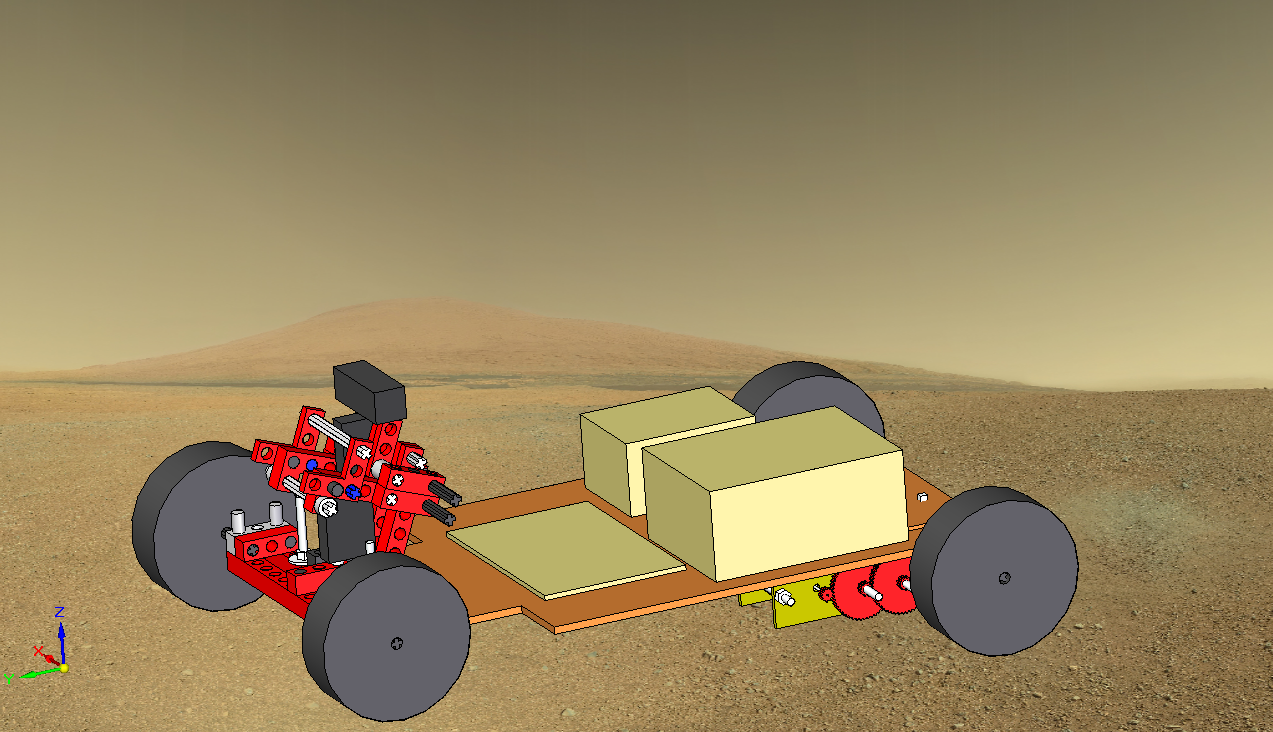
\includegraphics[width=\linewidth]{conceptkeuze-ontwerp/mechanisch/auto-resultaat.png}
 \caption{3D-model van het wagentje gemaakt met Solid Edge.}
 \label{image:auto-resultaat}
\end{figure}

De bodemplaat wordt schuin gemonteerd op beide assen en ligt hoger aan de 
achterkant. De plaat staat schuin omdat de motor en overbrenging aan de 
onderkant gemonteerd zijn. Hierdoor is er genoeg plaats over aan de bovenkant 
voor de elektronica en kunnen de tandwielen de draden niet beschadigen. 
Op de bovenkant van de bodemplaat komt de Arduino, de batterij en het Printed 
Circuit Board (PCB). Het gewicht wordt hierbij zo centraal mogelijk geplaatst, 
zodat het stuurmechanisme nog genoeg grip heeft om de koers van de wagen te 
wijzigen, zonder daarbij te veel weerstand te veroorzaken voor de servomotor. 
Bij een te hoge weerstand zou de servomotor de wielen niet op tijd kunnen 
draaien en zou de wagen de muur raken.

Het voordeel aan dit ontwerp is dat de stabiliteit, snelheid en wendbaarheid 
geoptimaliseerd worden. 

 
\subsection{Elektronisch}

 
\subsection{AI}
De aansturende software op de Arduinocontroler laat de radarsensor afwisselend links, vooruit en rechts de afstand meten. Afhankelijk van de gemeten waarden stuurt de software het wagentje bij.
Van zodra voor de afstandssensor vooruit een muur opmerkt, stopt het wagentje. Afhankelijk van de gemeten waarden links en rechts, weet de software aan welke kant het volgende deel van het traject zich bevindt.
Indien zich aan beide kanten een muur bevindt, is de rover op de bestemming aangekomen en knippert een LED.
Wanneer er voor het wagentje geen muur staat en de waarden links en rechts indiceren dat het wagentje zich tussen twee muren bevindt, maar dat de ene muur dichterbij is dan de andere, stuurt de software de baan van de wagen bij.

De software bestaat uit verschillende klassen die abstractie maken van de hardwarespecifieke commando's om de sensoren in te lezen en de actoren aan te sturen.
Zo is er een MyServo-, LedOutput-, Motor-, DistanceSensor-, MusicPlayer en PushButtonklasse. Deze laatste twee werden niet gebruikt in het uiteindelijke ontwerp, maar het programmeren van de skeletten gebeurde reeds in een eerste fase van het project.

De DrivingManagerklasse is de centrale unit van waaruit de wagen aangestuurd wordt. Deze klasse neemt de beslissingen zoals hierboven beschreven. 
DrivingManager kan de objecten manipuleren door middel van duidelijke commando's, zonder details over de onderliggende commando's. 
De methode setMotorSpeed in de klasse Motor regelt zo bijvoorbeeld de snelheid van de motoren en de staat van de relais, zodat ook achteruit gereden kan worden.

Om het testen van de aparte sensoren en actoren te vergemakkelijken, staan er ook enkele demo's in de DrivingManager-klasse. Deze zijn bedoeld om de specifieke elementen te testen. 
De methode radarDemo roteert bijvoorbeeld de servo waarop de afstandssensor gemonteerd is en de ingelezen waarden van de afstandssensor worden dan (geconverteerd naar centimeter) doorgestuurd via de Serial Monitor. Op die manier kan dit onderdeel gemakkelijker onderzocht worden op problemen als het aangesloten is aan de Arduino IDE\footnote{IDE: Integrated Development Environment (geïntegreerde ontwikkelomgeving).}.

De volledige code bevindt zich in Bijlage~\ref{bijlage:programma-code}.
